\documentclass[aspectratio=169]{beamer}
    \usepackage[utf8]{inputenc}
    \usetheme{Warsaw}

    \title{Pr\'esentation projet Technologie Web : INSAClash}
    \author{LAINE Bastien \\POINTIN Damien}
    \institute{G\'enie Math\'ematique - INSA Rouen}

    \begin{document}

    \begin{frame}
    \titlepage
    \end{frame}

    \begin{frame}
        \frametitle{Pr\'esentation d'INSAClash}
        \framesubtitle{Clash of Clans-like}
        Clash of Clans...
        \begin{center}
            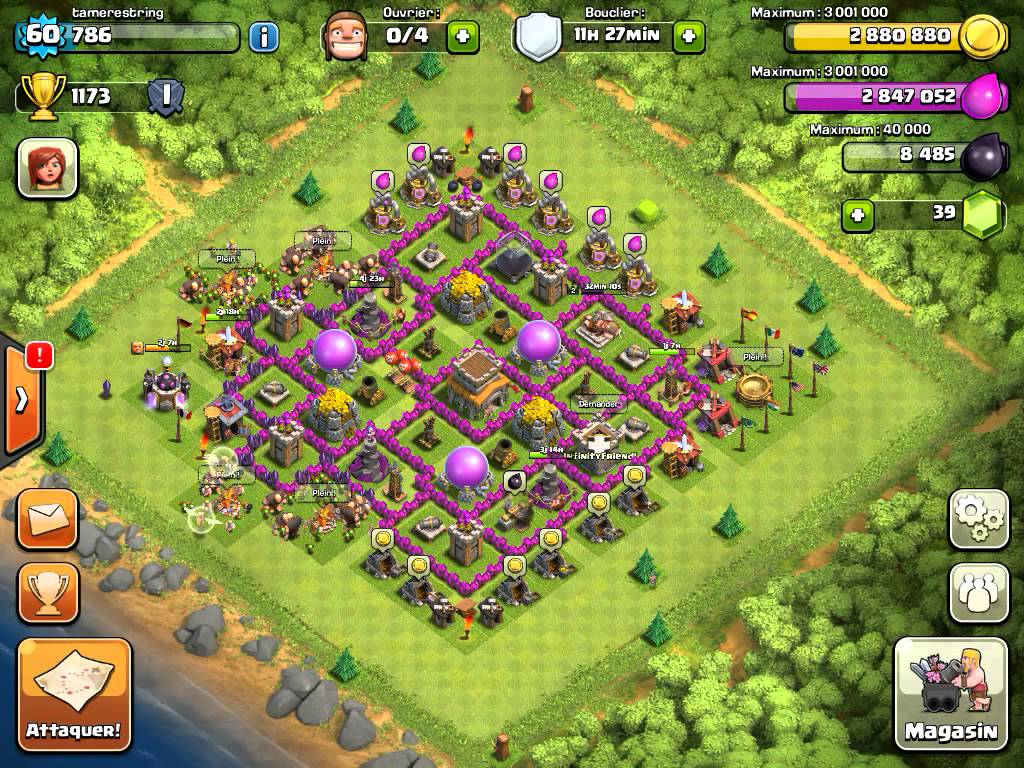
\includegraphics[scale=0.2]{images/clashOfClan.jpg}
        \end{center}
    \end{frame}

    \begin{frame}
        \frametitle{Pr\'esentation d'INSAClash}
        \framesubtitle{Clash of Clans-like}
        \ldots Avec des règles simplifi\'es
        \begin{itemize}
            \item Absence de \textbf{clans}
            \item Simplification de la gestion des \textbf{arm\'ees} et des \textbf{bâtiments}
            \item Simplification de la gestion des \textbf{ressources}
        \end{itemize}
    \end{frame}

    \begin{frame}
        \frametitle{D\'etails des lots}
        Projets en plusieurs lots:
        \begin{itemize}
            \item Lot \#1: 02/02/2016\\
                \begin{itemize}
                    \item Modèle
                \end{itemize}
            \item Lot \#2: 23/02/2016
                \begin{itemize}
                    \item Interface Web v1 (Gestion individuelle)
                    \item Stockage
                \end{itemize}
            \item Lot \#3: 15/03/2016
                \begin{itemize}
                    \item Interface Web v2 (Interaction multijoueur - Combats)
                \end{itemize}
        \end{itemize}
    \end{frame}

    \begin{frame}
        \frametitle{Analyse descendante - 1}
        \framesubtitle{Analyse descendante générale}
        \begin{center}
            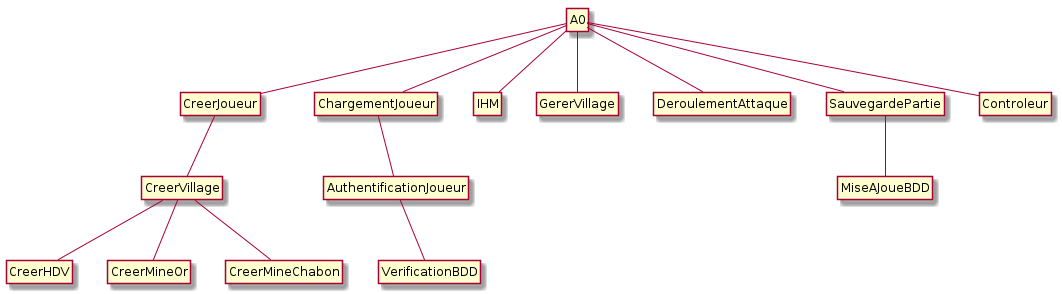
\includegraphics[scale=0.3]{graph/analyseDescendante.png}
        \end{center}
    \end{frame}
    \begin{frame}
        \frametitle{Analyse descendante - 2}
        \framesubtitle{Zoom: IHM}
        \begin{center}
            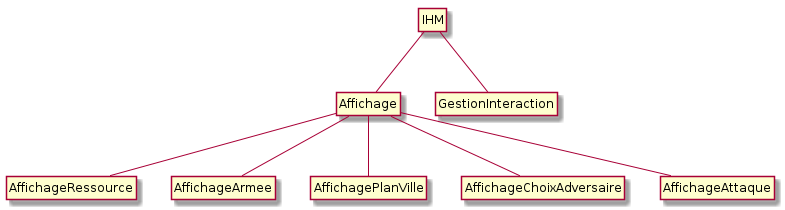
\includegraphics[scale=0.3]{graph/IHM.png}
        \end{center}
    \end{frame}
    \begin{frame}
        \frametitle{Analyse descendante - 3}
        \framesubtitle{Zoom: Deroulement Attaque}
        \begin{center}
            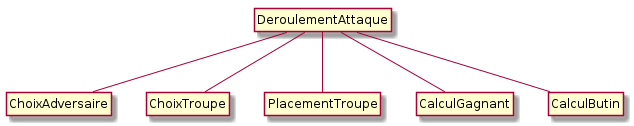
\includegraphics[scale=0.3]{graph/DeroulementAttaque.png}
        \end{center}
    \end{frame}
    \begin{frame}
        \frametitle{Analyse descendante - 4}
        \framesubtitle{Zoom: Gestion Village}
        \begin{center}
            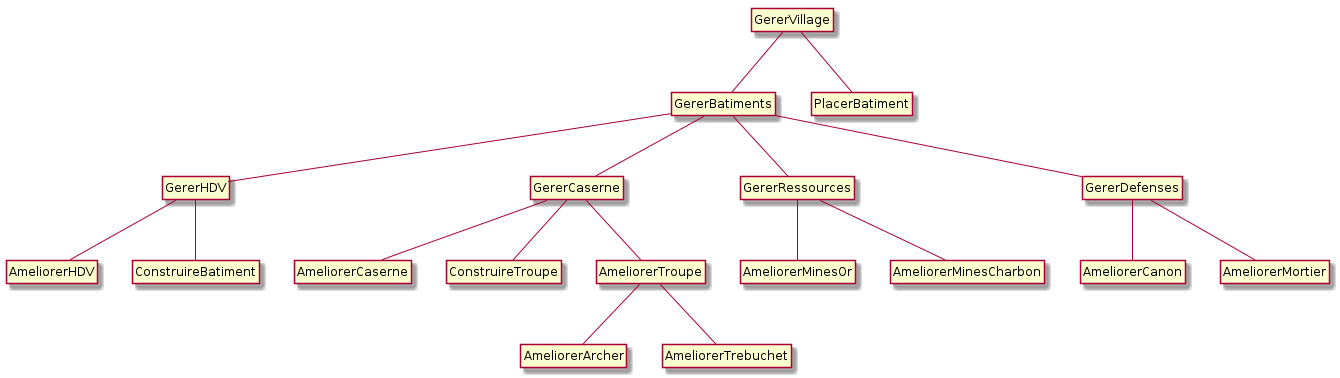
\includegraphics[scale=0.2]{graph/GestionVillage.png}
        \end{center}
    \end{frame}

    \begin{frame}
        \frametitle{Orient\'e objet}
        \framesubtitle{Utilit\'e de l'orient\'e objet}
        Est-il judicieux d'utiliser un paradigme objet ?
    \end{frame}
    \begin{frame}
        \frametitle{Orient\'e objet}
        \framesubtitle{Diagramme de classes}
        \includegraphics[scale=0.4]{graph/Classes.png}
    \end{frame}

    \begin{frame}
        \frametitle{Technologies \& Méthodologies}
        \framesubtitle{Technologies}
        Technologies employées:
        \begin{itemize}
            \item Modèle : JAVA
            \item Interface Web : J2EE
            \item Stockage: MySQL
        \end{itemize}
    \end{frame}
    \begin{frame}
        \frametitle{Technologies \& Méthodologies}
        \framesubtitle{Méthodologies}
        Méthodologies employées:
        \begin{itemize}
            \item Eclipse
            \item Git
            \item Latex
            \item PlantUML
            \item Script BASH pour génération diagramme de classes
        \end{itemize}
    \end{frame}

    \begin{frame}
        \begin{center}
            Questions?
        \end{center}
    \end{frame}

\end{document}
